%
% General Runtimes
%
\section{General Runtimes}

\subsection{total}
total is a general runtime.

See plots: \ref{plot:RANDOM_100_500 - BARABASI_ALBERT_GROWTH_10_2.z.runtimes.0.all}, \ref{plot:RANDOM_100_500 - BARABASI_ALBERT_GROWTH_10_2.z.runtimes.0.all.CDF}, \ref{plot:RANDOM_100_500 - BARABASI_ALBERT_GROWTH_10_2.z.runtimes.1.total}, \ref{plot:RANDOM_100_500 - BARABASI_ALBERT_GROWTH_10_2.z.runtimes.1.total.CDF}.

%
% value table of total
%
\begin{tabular}{|l||l|}
\hline
	\textbf{Timestamp} & \textbf{Average} \\ \hline
	0 & 0.1283 \\ \hline
	1 & 0.03622 \\ \hline
	2 & 0.02207 \\ \hline
	3 & 0.01295 \\ \hline
	4 & 0.0116 \\ \hline
	5 & 0.01284 \\ \hline
	6 & 0.01656 \\ \hline
	7 & 0.01962 \\ \hline
	8 & 0.01908 \\ \hline
	9 & 0.0213 \\ \hline
	10 & 0.02265 \\ \hline
	11 & 0.0241 \\ \hline
	12 & 0.02508 \\ \hline
	13 & 0.0256 \\ \hline
	14 & 0.03143 \\ \hline
	15 & 0.02396 \\ \hline
	16 & 0.02621 \\ \hline
	17 & 0.02403 \\ \hline
	18 & 0.02601 \\ \hline
	19 & 0.02815 \\ \hline
	20 & 0.03089 \\ \hline
	21 & 0.03083 \\ \hline
	22 & 0.03129 \\ \hline
	23 & 0.03712 \\ \hline
	24 & 0.03658 \\ \hline
	25 & 0.03474 \\ \hline
	26 & 0.04277 \\ \hline
	27 & 0.04217 \\ \hline
	28 & 0.04902 \\ \hline
	29 & 0.04852 \\ \hline
	30 & 0.05137 \\ \hline
	31 & 0.06068 \\ \hline
	32 & 0.05426 \\ \hline
	33 & 0.05942 \\ \hline
	34 & 0.06162 \\ \hline
	35 & 0.06156 \\ \hline
	36 & 0.06291 \\ \hline
	37 & 0.0711 \\ \hline
	38 & 0.08362 \\ \hline
	39 & 0.07326 \\ \hline
	40 & 0.07739 \\ \hline
	41 & 0.0804 \\ \hline
	42 & 0.08084 \\ \hline
	43 & 0.08255 \\ \hline
	44 & 0.08394 \\ \hline
	45 & 0.0871 \\ \hline
\end{tabular}
\begin{tabular}{|l||l|}
\hline
	\textbf{Timestamp} & \textbf{Average} \\ \hline
	46 & 0.08901 \\ \hline
	47 & 0.09574 \\ \hline
	48 & 0.09986 \\ \hline
	49 & 0.1028 \\ \hline
	50 & 0.1023 \\ \hline
\end{tabular}

\subsection{overhead}
overhead is a general runtime.

See plot: \ref{plot:RANDOM_100_500 - BARABASI_ALBERT_GROWTH_10_2.z.runtimes.0.all}, \ref{plot:RANDOM_100_500 - BARABASI_ALBERT_GROWTH_10_2.z.runtimes.0.all.CDF}.

%
% value table of overhead
%
\begin{tabular}{|l||l|}
\hline
	\textbf{Timestamp} & \textbf{Average} \\ \hline
	0 & 0.00654 \\ \hline
	1 & 0.00344 \\ \hline
	2 & 0.00253 \\ \hline
	3 & 0.00212 \\ \hline
	4 & 0.00142 \\ \hline
	5 & 0.00152 \\ \hline
	6 & 0.00148 \\ \hline
	7 & 0.00222 \\ \hline
	8 & 0.00178 \\ \hline
	9 & 0.00186 \\ \hline
	10 & 0.00195 \\ \hline
	11 & 0.00235 \\ \hline
	12 & 0.00197 \\ \hline
	13 & 0.00223 \\ \hline
	14 & 0.00235 \\ \hline
	15 & 0.00106 \\ \hline
	16 & 9.21E-4 \\ \hline
	17 & 6.8E-4 \\ \hline
	18 & 7.97E-4 \\ \hline
	19 & 0.00104 \\ \hline
	20 & 6.87E-4 \\ \hline
	21 & 7.61E-4 \\ \hline
	22 & 7.67E-4 \\ \hline
	23 & 6.6E-4 \\ \hline
	24 & 6.71E-4 \\ \hline
	25 & 5.77E-4 \\ \hline
	26 & 7.29E-4 \\ \hline
	27 & 7.31E-4 \\ \hline
	28 & 7.55E-4 \\ \hline
	29 & 6.26E-4 \\ \hline
	30 & 6.21E-4 \\ \hline
	31 & 5.7E-4 \\ \hline
	32 & 3.73E-4 \\ \hline
	33 & 5.46E-4 \\ \hline
	34 & 4.74E-4 \\ \hline
	35 & 4.44E-4 \\ \hline
	36 & 4.34E-4 \\ \hline
	37 & 4.76E-4 \\ \hline
	38 & 6.97E-4 \\ \hline
	39 & 4.08E-4 \\ \hline
	40 & 3.83E-4 \\ \hline
	41 & 4.18E-4 \\ \hline
	42 & 4.36E-4 \\ \hline
	43 & 4.16E-4 \\ \hline
	44 & 4.57E-4 \\ \hline
	45 & 3.89E-4 \\ \hline
\end{tabular}
\begin{tabular}{|l||l|}
\hline
	\textbf{Timestamp} & \textbf{Average} \\ \hline
	46 & 4.12E-4 \\ \hline
	47 & 3.97E-4 \\ \hline
	48 & 4.59E-4 \\ \hline
	49 & 3.93E-4 \\ \hline
	50 & 3.93E-4 \\ \hline
\end{tabular}

\subsection{metrics}
metrics is a general runtime.

See plots: \ref{plot:RANDOM_100_500 - BARABASI_ALBERT_GROWTH_10_2.z.runtimes.0.all}, \ref{plot:RANDOM_100_500 - BARABASI_ALBERT_GROWTH_10_2.z.runtimes.0.all.CDF}, \ref{plot:RANDOM_100_500 - BARABASI_ALBERT_GROWTH_10_2.z.runtimes.3.allMetrics}, \ref{plot:RANDOM_100_500 - BARABASI_ALBERT_GROWTH_10_2.z.runtimes.3.allMetrics.CDF}.

%
% value table of metrics
%
\begin{tabular}{|l||l|}
\hline
	\textbf{Timestamp} & \textbf{Average} \\ \hline
	0 & 0.07118 \\ \hline
	1 & 0.0195 \\ \hline
	2 & 0.0162 \\ \hline
	3 & 0.00852 \\ \hline
	4 & 0.00838 \\ \hline
	5 & 0.00962 \\ \hline
	6 & 0.01302 \\ \hline
	7 & 0.01501 \\ \hline
	8 & 0.01585 \\ \hline
	9 & 0.01766 \\ \hline
	10 & 0.01903 \\ \hline
	11 & 0.01992 \\ \hline
	12 & 0.02123 \\ \hline
	13 & 0.02147 \\ \hline
	14 & 0.02671 \\ \hline
	15 & 0.02085 \\ \hline
	16 & 0.02321 \\ \hline
	17 & 0.02232 \\ \hline
	18 & 0.02427 \\ \hline
	19 & 0.02575 \\ \hline
	20 & 0.02929 \\ \hline
	21 & 0.0291 \\ \hline
	22 & 0.02952 \\ \hline
	23 & 0.03565 \\ \hline
	24 & 0.03499 \\ \hline
	25 & 0.03335 \\ \hline
	26 & 0.04108 \\ \hline
	27 & 0.04029 \\ \hline
	28 & 0.04737 \\ \hline
	29 & 0.04688 \\ \hline
	30 & 0.04909 \\ \hline
	31 & 0.059 \\ \hline
	32 & 0.05318 \\ \hline
	33 & 0.05801 \\ \hline
	34 & 0.06008 \\ \hline
	35 & 0.06027 \\ \hline
	36 & 0.06165 \\ \hline
	37 & 0.06975 \\ \hline
	38 & 0.08154 \\ \hline
	39 & 0.07212 \\ \hline
	40 & 0.07628 \\ \hline
	41 & 0.07915 \\ \hline
	42 & 0.07953 \\ \hline
	43 & 0.08132 \\ \hline
	44 & 0.0826 \\ \hline
	45 & 0.08598 \\ \hline
\end{tabular}
\begin{tabular}{|l||l|}
\hline
	\textbf{Timestamp} & \textbf{Average} \\ \hline
	46 & 0.08782 \\ \hline
	47 & 0.09445 \\ \hline
	48 & 0.09838 \\ \hline
	49 & 0.1016 \\ \hline
	50 & 0.1012 \\ \hline
\end{tabular}

\subsection{graphUpdate}
graphUpdate is a general runtime.

See plots: \ref{plot:RANDOM_100_500 - BARABASI_ALBERT_GROWTH_10_2.z.runtimes.0.all}, \ref{plot:RANDOM_100_500 - BARABASI_ALBERT_GROWTH_10_2.z.runtimes.0.all.CDF}, \ref{plot:RANDOM_100_500 - BARABASI_ALBERT_GROWTH_10_2.z.runtimes.4.graphUpdate.CDF}.

%
% value table of graphUpdate
%
\begin{tabular}{|l||l|}
\hline
	\textbf{Timestamp} & \textbf{Average} \\ \hline
	0 & 0 \\ \hline
	1 & 4.17E-4 \\ \hline
	2 & 6.2E-4 \\ \hline
	3 & 4.44E-4 \\ \hline
	4 & 3.11E-4 \\ \hline
	5 & 3.18E-4 \\ \hline
	6 & 3.16E-4 \\ \hline
	7 & 4.52E-4 \\ \hline
	8 & 4.04E-4 \\ \hline
	9 & 4.49E-4 \\ \hline
	10 & 4.37E-4 \\ \hline
	11 & 4.73E-4 \\ \hline
	12 & 4.46E-4 \\ \hline
	13 & 4.96E-4 \\ \hline
	14 & 7.28E-4 \\ \hline
	15 & 4.25E-4 \\ \hline
	16 & 4.34E-4 \\ \hline
	17 & 2.56E-4 \\ \hline
	18 & 3.12E-4 \\ \hline
	19 & 3.92E-4 \\ \hline
	20 & 2.74E-4 \\ \hline
	21 & 3.2E-4 \\ \hline
	22 & 3.16E-4 \\ \hline
	23 & 2.29E-4 \\ \hline
	24 & 2.71E-4 \\ \hline
	25 & 2.17E-4 \\ \hline
	26 & 2.75E-4 \\ \hline
	27 & 2.6E-4 \\ \hline
	28 & 2.6E-4 \\ \hline
	29 & 2.19E-4 \\ \hline
	30 & 7.84E-4 \\ \hline
	31 & 2.87E-4 \\ \hline
	32 & 1.96E-4 \\ \hline
	33 & 2.6E-4 \\ \hline
	34 & 2.53E-4 \\ \hline
	35 & 2.48E-4 \\ \hline
	36 & 2.61E-4 \\ \hline
	37 & 2.56E-4 \\ \hline
	38 & 3.63E-4 \\ \hline
	39 & 2.06E-4 \\ \hline
	40 & 1.97E-4 \\ \hline
	41 & 2.35E-4 \\ \hline
	42 & 2.75E-4 \\ \hline
	43 & 2.36E-4 \\ \hline
	44 & 2.64E-4 \\ \hline
	45 & 2.08E-4 \\ \hline
\end{tabular}
\begin{tabular}{|l||l|}
\hline
	\textbf{Timestamp} & \textbf{Average} \\ \hline
	46 & 2.36E-4 \\ \hline
	47 & 2.12E-4 \\ \hline
	48 & 2.64E-4 \\ \hline
	49 & 2.35E-4 \\ \hline
	50 & 2.14E-4 \\ \hline
\end{tabular}

\subsection{batchGeneration}
batchGeneration is a general runtime.

See plots: \ref{plot:RANDOM_100_500 - BARABASI_ALBERT_GROWTH_10_2.z.runtimes.0.all}, \ref{plot:RANDOM_100_500 - BARABASI_ALBERT_GROWTH_10_2.z.runtimes.0.all.CDF}, \ref{plot:RANDOM_100_500 - BARABASI_ALBERT_GROWTH_10_2.z.runtimes.5.batchGeneration.CDF}.

%
% value table of batchGeneration
%
\begin{tabular}{|l||l|}
\hline
	\textbf{Timestamp} & \textbf{Average} \\ \hline
	0 & 0 \\ \hline
	1 & 0.01286 \\ \hline
	2 & 0.00272 \\ \hline
	3 & 0.00186 \\ \hline
	4 & 0.00149 \\ \hline
	5 & 0.00138 \\ \hline
	6 & 0.00175 \\ \hline
	7 & 0.00193 \\ \hline
	8 & 0.00104 \\ \hline
	9 & 0.00133 \\ \hline
	10 & 0.00123 \\ \hline
	11 & 0.00135 \\ \hline
	12 & 0.00142 \\ \hline
	13 & 0.0014 \\ \hline
	14 & 0.00164 \\ \hline
	15 & 0.00162 \\ \hline
	16 & 0.00164 \\ \hline
	17 & 7.69E-4 \\ \hline
	18 & 6.32E-4 \\ \hline
	19 & 9.67E-4 \\ \hline
	20 & 6.45E-4 \\ \hline
	21 & 6.45E-4 \\ \hline
	22 & 6.93E-4 \\ \hline
	23 & 5.86E-4 \\ \hline
	24 & 6.51E-4 \\ \hline
	25 & 5.97E-4 \\ \hline
	26 & 6.92E-4 \\ \hline
	27 & 8.91E-4 \\ \hline
	28 & 6.27E-4 \\ \hline
	29 & 7.91E-4 \\ \hline
	30 & 8.78E-4 \\ \hline
	31 & 8.15E-4 \\ \hline
	32 & 5.14E-4 \\ \hline
	33 & 5.97E-4 \\ \hline
	34 & 8.19E-4 \\ \hline
	35 & 5.97E-4 \\ \hline
	36 & 5.67E-4 \\ \hline
	37 & 6.15E-4 \\ \hline
	38 & 0.00102 \\ \hline
	39 & 5.25E-4 \\ \hline
	40 & 5.22E-4 \\ \hline
	41 & 6E-4 \\ \hline
	42 & 6.01E-4 \\ \hline
	43 & 5.85E-4 \\ \hline
	44 & 6.15E-4 \\ \hline
	45 & 5.26E-4 \\ \hline
\end{tabular}
\begin{tabular}{|l||l|}
\hline
	\textbf{Timestamp} & \textbf{Average} \\ \hline
	46 & 5.42E-4 \\ \hline
	47 & 6.83E-4 \\ \hline
	48 & 7.61E-4 \\ \hline
	49 & 5.95E-4 \\ \hline
	50 & 5.71E-4 \\ \hline
\end{tabular}

\subsection{profiler}
profiler is a general runtime.

See plot: \ref{plot:RANDOM_100_500 - BARABASI_ALBERT_GROWTH_10_2.z.runtimes.0.all}, \ref{plot:RANDOM_100_500 - BARABASI_ALBERT_GROWTH_10_2.z.runtimes.0.all.CDF}.

%
% value table of profiler
%
\begin{tabular}{|l||l|}
\hline
	\textbf{Timestamp} & \textbf{Average} \\ \hline
	0 & 0 \\ \hline
	1 & 0 \\ \hline
	2 & 0 \\ \hline
	3 & 0 \\ \hline
	4 & 0 \\ \hline
	5 & 0 \\ \hline
	6 & 0 \\ \hline
	7 & 0 \\ \hline
	8 & 0 \\ \hline
	9 & 0 \\ \hline
	10 & 0 \\ \hline
	11 & 0 \\ \hline
	12 & 0 \\ \hline
	13 & 0 \\ \hline
	14 & 0 \\ \hline
	15 & 0 \\ \hline
	16 & 0 \\ \hline
	17 & 0 \\ \hline
	18 & 0 \\ \hline
	19 & 0 \\ \hline
	20 & 0 \\ \hline
	21 & 0 \\ \hline
	22 & 0 \\ \hline
	23 & 0 \\ \hline
	24 & 0 \\ \hline
	25 & 0 \\ \hline
	26 & 0 \\ \hline
	27 & 0 \\ \hline
	28 & 0 \\ \hline
	29 & 0 \\ \hline
	30 & 0 \\ \hline
	31 & 0 \\ \hline
	32 & 0 \\ \hline
	33 & 0 \\ \hline
	34 & 0 \\ \hline
	35 & 0 \\ \hline
	36 & 0 \\ \hline
	37 & 0 \\ \hline
	38 & 0 \\ \hline
	39 & 0 \\ \hline
	40 & 0 \\ \hline
	41 & 0 \\ \hline
	42 & 0 \\ \hline
	43 & 0 \\ \hline
	44 & 0 \\ \hline
	45 & 0 \\ \hline
\end{tabular}
\begin{tabular}{|l||l|}
\hline
	\textbf{Timestamp} & \textbf{Average} \\ \hline
	46 & 0 \\ \hline
	47 & 0 \\ \hline
	48 & 0 \\ \hline
	49 & 0 \\ \hline
	50 & 0 \\ \hline
\end{tabular}

\subsection{hotswap}
hotswap is a general runtime.

See plot: \ref{plot:RANDOM_100_500 - BARABASI_ALBERT_GROWTH_10_2.z.runtimes.0.all}, \ref{plot:RANDOM_100_500 - BARABASI_ALBERT_GROWTH_10_2.z.runtimes.0.all.CDF}.

%
% value table of hotswap
%
\begin{tabular}{|l||l|}
\hline
	\textbf{Timestamp} & \textbf{Average} \\ \hline
	0 & 0 \\ \hline
	1 & 0 \\ \hline
	2 & 0 \\ \hline
	3 & 0 \\ \hline
	4 & 0 \\ \hline
	5 & 0 \\ \hline
	6 & 0 \\ \hline
	7 & 0 \\ \hline
	8 & 0 \\ \hline
	9 & 0 \\ \hline
	10 & 0 \\ \hline
	11 & 0 \\ \hline
	12 & 0 \\ \hline
	13 & 0 \\ \hline
	14 & 0 \\ \hline
	15 & 0 \\ \hline
	16 & 0 \\ \hline
	17 & 0 \\ \hline
	18 & 0 \\ \hline
	19 & 0 \\ \hline
	20 & 0 \\ \hline
	21 & 0 \\ \hline
	22 & 0 \\ \hline
	23 & 0 \\ \hline
	24 & 0 \\ \hline
	25 & 0 \\ \hline
	26 & 0 \\ \hline
	27 & 0 \\ \hline
	28 & 0 \\ \hline
	29 & 0 \\ \hline
	30 & 0 \\ \hline
	31 & 0 \\ \hline
	32 & 0 \\ \hline
	33 & 0 \\ \hline
	34 & 0 \\ \hline
	35 & 0 \\ \hline
	36 & 0 \\ \hline
	37 & 0 \\ \hline
	38 & 0 \\ \hline
	39 & 0 \\ \hline
	40 & 0 \\ \hline
	41 & 0 \\ \hline
	42 & 0 \\ \hline
	43 & 0 \\ \hline
	44 & 0 \\ \hline
	45 & 0 \\ \hline
\end{tabular}
\begin{tabular}{|l||l|}
\hline
	\textbf{Timestamp} & \textbf{Average} \\ \hline
	46 & 0 \\ \hline
	47 & 0 \\ \hline
	48 & 0 \\ \hline
	49 & 0 \\ \hline
	50 & 0 \\ \hline
\end{tabular}

\subsection{graphGeneration}
graphGeneration is a general runtime.

%
% value table of graphGeneration
%
\begin{tabular}{|l||l|}
\hline
	\textbf{Timestamp} & \textbf{Average} \\ \hline
	0 & 0.05053 \\ \hline
	1 & 0 \\ \hline
	2 & 0 \\ \hline
	3 & 0 \\ \hline
	4 & 0 \\ \hline
	5 & 0 \\ \hline
	6 & 0 \\ \hline
	7 & 0 \\ \hline
	8 & 0 \\ \hline
	9 & 0 \\ \hline
	10 & 0 \\ \hline
	11 & 0 \\ \hline
	12 & 0 \\ \hline
	13 & 0 \\ \hline
	14 & 0 \\ \hline
	15 & 0 \\ \hline
	16 & 0 \\ \hline
	17 & 0 \\ \hline
	18 & 0 \\ \hline
	19 & 0 \\ \hline
	20 & 0 \\ \hline
	21 & 0 \\ \hline
	22 & 0 \\ \hline
	23 & 0 \\ \hline
	24 & 0 \\ \hline
	25 & 0 \\ \hline
	26 & 0 \\ \hline
	27 & 0 \\ \hline
	28 & 0 \\ \hline
	29 & 0 \\ \hline
	30 & 0 \\ \hline
	31 & 0 \\ \hline
	32 & 0 \\ \hline
	33 & 0 \\ \hline
	34 & 0 \\ \hline
	35 & 0 \\ \hline
	36 & 0 \\ \hline
	37 & 0 \\ \hline
	38 & 0 \\ \hline
	39 & 0 \\ \hline
	40 & 0 \\ \hline
	41 & 0 \\ \hline
	42 & 0 \\ \hline
	43 & 0 \\ \hline
	44 & 0 \\ \hline
	45 & 0 \\ \hline
\end{tabular}
\begin{tabular}{|l||l|}
\hline
	\textbf{Timestamp} & \textbf{Average} \\ \hline
	46 & 0 \\ \hline
	47 & 0 \\ \hline
	48 & 0 \\ \hline
	49 & 0 \\ \hline
	50 & 0 \\ \hline
\end{tabular}

\subsection{recommendation}
recommendation is a general runtime.

See plot: \ref{plot:RANDOM_100_500 - BARABASI_ALBERT_GROWTH_10_2.z.runtimes.0.all}, \ref{plot:RANDOM_100_500 - BARABASI_ALBERT_GROWTH_10_2.z.runtimes.0.all.CDF}.

%
% value table of recommendation
%
\begin{tabular}{|l||l|}
\hline
	\textbf{Timestamp} & \textbf{Average} \\ \hline
	0 & 0 \\ \hline
	1 & 0 \\ \hline
	2 & 0 \\ \hline
	3 & 0 \\ \hline
	4 & 0 \\ \hline
	5 & 0 \\ \hline
	6 & 0 \\ \hline
	7 & 0 \\ \hline
	8 & 0 \\ \hline
	9 & 0 \\ \hline
	10 & 0 \\ \hline
	11 & 0 \\ \hline
	12 & 0 \\ \hline
	13 & 0 \\ \hline
	14 & 0 \\ \hline
	15 & 0 \\ \hline
	16 & 0 \\ \hline
	17 & 0 \\ \hline
	18 & 0 \\ \hline
	19 & 0 \\ \hline
	20 & 0 \\ \hline
	21 & 0 \\ \hline
	22 & 0 \\ \hline
	23 & 0 \\ \hline
	24 & 0 \\ \hline
	25 & 0 \\ \hline
	26 & 0 \\ \hline
	27 & 0 \\ \hline
	28 & 0 \\ \hline
	29 & 0 \\ \hline
	30 & 0 \\ \hline
	31 & 0 \\ \hline
	32 & 0 \\ \hline
	33 & 0 \\ \hline
	34 & 0 \\ \hline
	35 & 0 \\ \hline
	36 & 0 \\ \hline
	37 & 0 \\ \hline
	38 & 0 \\ \hline
	39 & 0 \\ \hline
	40 & 0 \\ \hline
	41 & 0 \\ \hline
	42 & 0 \\ \hline
	43 & 0 \\ \hline
	44 & 0 \\ \hline
	45 & 0 \\ \hline
\end{tabular}
\begin{tabular}{|l||l|}
\hline
	\textbf{Timestamp} & \textbf{Average} \\ \hline
	46 & 0 \\ \hline
	47 & 0 \\ \hline
	48 & 0 \\ \hline
	49 & 0 \\ \hline
	50 & 0 \\ \hline
\end{tabular}

\subsection{sum}
sum is a general runtime.

See plot: \ref{plot:RANDOM_100_500 - BARABASI_ALBERT_GROWTH_10_2.z.runtimes.0.all}, \ref{plot:RANDOM_100_500 - BARABASI_ALBERT_GROWTH_10_2.z.runtimes.0.all.CDF}.

%
% value table of sum
%
\begin{tabular}{|l||l|}
\hline
	\textbf{Timestamp} & \textbf{Average} \\ \hline
	0 & 0.1217 \\ \hline
	1 & 0.03278 \\ \hline
	2 & 0.01954 \\ \hline
	3 & 0.01083 \\ \hline
	4 & 0.01019 \\ \hline
	5 & 0.01132 \\ \hline
	6 & 0.01508 \\ \hline
	7 & 0.0174 \\ \hline
	8 & 0.0173 \\ \hline
	9 & 0.01944 \\ \hline
	10 & 0.0207 \\ \hline
	11 & 0.02174 \\ \hline
	12 & 0.0231 \\ \hline
	13 & 0.02336 \\ \hline
	14 & 0.02908 \\ \hline
	15 & 0.0229 \\ \hline
	16 & 0.02529 \\ \hline
	17 & 0.02335 \\ \hline
	18 & 0.02521 \\ \hline
	19 & 0.02711 \\ \hline
	20 & 0.03021 \\ \hline
	21 & 0.03007 \\ \hline
	22 & 0.03053 \\ \hline
	23 & 0.03646 \\ \hline
	24 & 0.03591 \\ \hline
	25 & 0.03416 \\ \hline
	26 & 0.04204 \\ \hline
	27 & 0.04144 \\ \hline
	28 & 0.04826 \\ \hline
	29 & 0.04789 \\ \hline
	30 & 0.05075 \\ \hline
	31 & 0.06011 \\ \hline
	32 & 0.05388 \\ \hline
	33 & 0.05887 \\ \hline
	34 & 0.06115 \\ \hline
	35 & 0.06112 \\ \hline
	36 & 0.06248 \\ \hline
	37 & 0.07062 \\ \hline
	38 & 0.08292 \\ \hline
	39 & 0.07286 \\ \hline
	40 & 0.077 \\ \hline
	41 & 0.07998 \\ \hline
	42 & 0.08041 \\ \hline
	43 & 0.08214 \\ \hline
	44 & 0.08348 \\ \hline
	45 & 0.08671 \\ \hline
\end{tabular}
\begin{tabular}{|l||l|}
\hline
	\textbf{Timestamp} & \textbf{Average} \\ \hline
	46 & 0.0886 \\ \hline
	47 & 0.09535 \\ \hline
	48 & 0.0994 \\ \hline
	49 & 0.1024 \\ \hline
	50 & 0.1019 \\ \hline
\end{tabular}

\subsection{Plots}

% plot z.runtimes.0.all
\begin{figure} [h]
	\centering
	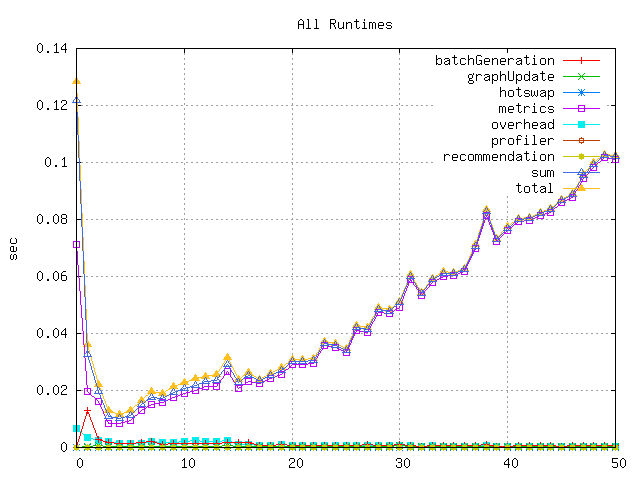
\includegraphics [scale=0.8] {plots/z.runtimes.0.all}
	\caption{z.runtimes.0.all}
	\label{plot:RANDOM_100_500 - BARABASI_ALBERT_GROWTH_10_2.z.runtimes.0.all}
\end{figure}

% plot z.runtimes.0.all.CDF
\begin{figure} [h]
	\centering
	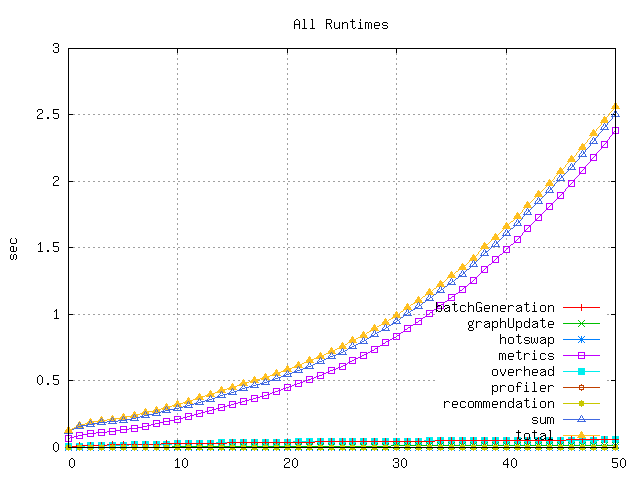
\includegraphics [scale=0.8] {plots/z.runtimes.0.all.CDF}
	\caption{z.runtimes.0.all.CDF}
	\label{plot:RANDOM_100_500 - BARABASI_ALBERT_GROWTH_10_2.z.runtimes.0.all.CDF}
\end{figure}

% plot z.runtimes.1.total
\begin{figure} [h]
	\centering
	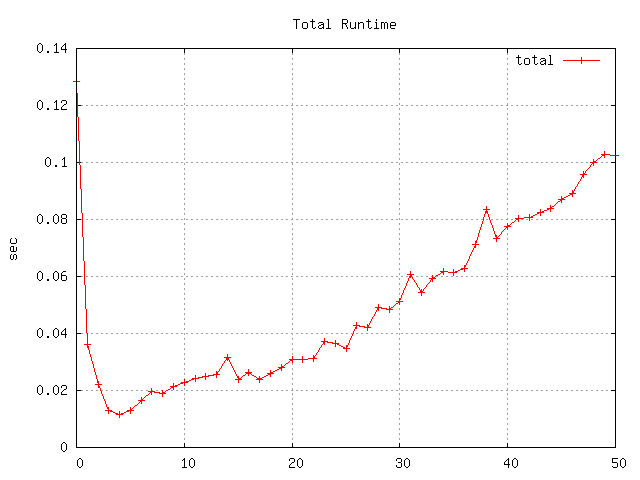
\includegraphics [scale=0.8] {plots/z.runtimes.1.total}
	\caption{z.runtimes.1.total}
	\label{plot:RANDOM_100_500 - BARABASI_ALBERT_GROWTH_10_2.z.runtimes.1.total}
\end{figure}

% plot z.runtimes.1.total.CDF
\begin{figure} [h]
	\centering
	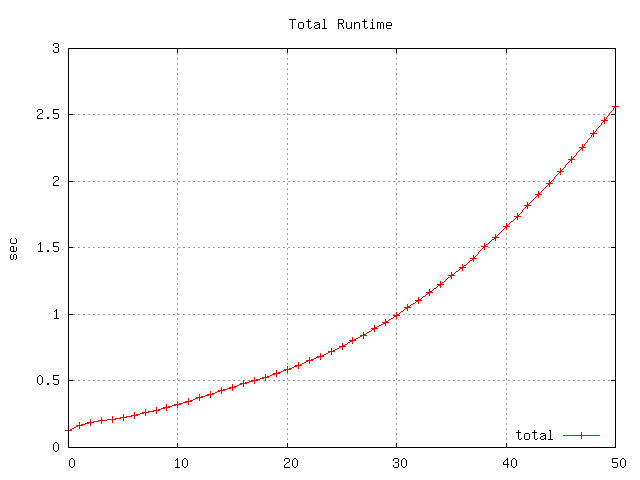
\includegraphics [scale=0.8] {plots/z.runtimes.1.total.CDF}
	\caption{z.runtimes.1.total.CDF}
	\label{plot:RANDOM_100_500 - BARABASI_ALBERT_GROWTH_10_2.z.runtimes.1.total.CDF}
\end{figure}

% plot z.runtimes.3.allMetrics
\begin{figure} [h]
	\centering
	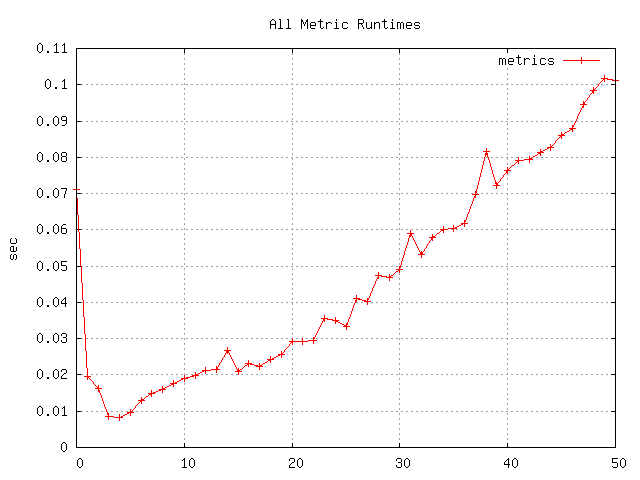
\includegraphics [scale=0.8] {plots/z.runtimes.3.allMetrics}
	\caption{z.runtimes.3.allMetrics}
	\label{plot:RANDOM_100_500 - BARABASI_ALBERT_GROWTH_10_2.z.runtimes.3.allMetrics}
\end{figure}

% plot z.runtimes.3.allMetrics.CDF
\begin{figure} [h]
	\centering
	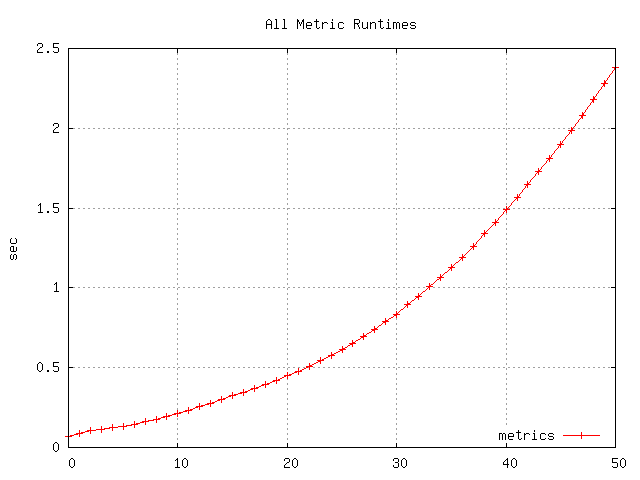
\includegraphics [scale=0.8] {plots/z.runtimes.3.allMetrics.CDF}
	\caption{z.runtimes.3.allMetrics.CDF}
	\label{plot:RANDOM_100_500 - BARABASI_ALBERT_GROWTH_10_2.z.runtimes.3.allMetrics.CDF}
\end{figure}

% plot z.runtimes.4.graphUpdate.CDF
\begin{figure} [h]
	\centering
	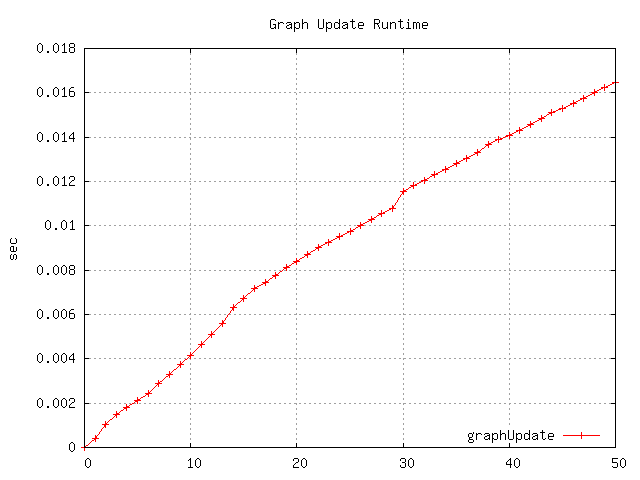
\includegraphics [scale=0.8] {plots/z.runtimes.4.graphUpdate.CDF}
	\caption{z.runtimes.4.graphUpdate.CDF}
	\label{plot:RANDOM_100_500 - BARABASI_ALBERT_GROWTH_10_2.z.runtimes.4.graphUpdate.CDF}
\end{figure}

% plot z.runtimes.5.batchGeneration.CDF
\begin{figure} [h]
	\centering
	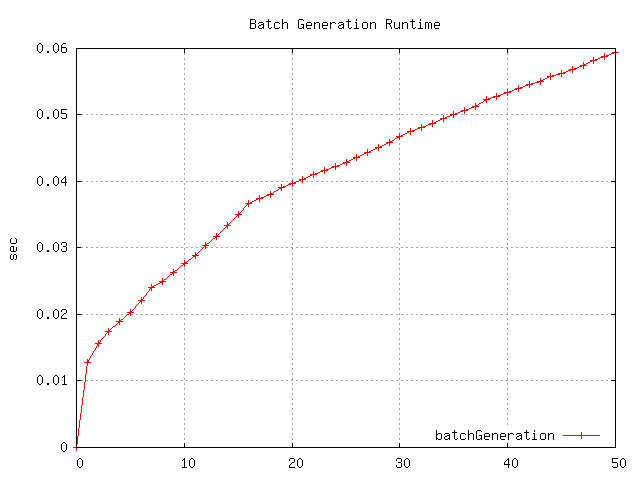
\includegraphics [scale=0.8] {plots/z.runtimes.5.batchGeneration.CDF}
	\caption{z.runtimes.5.batchGeneration.CDF}
	\label{plot:RANDOM_100_500 - BARABASI_ALBERT_GROWTH_10_2.z.runtimes.5.batchGeneration.CDF}
\end{figure}


% end of document
